\chapter{Metric, sự giãn nở và vũ trụ học bước đầu}

Ở cuối bài giảng trước, chúng ta đã đi tới một phương trình sóng bất biến Lorentz và đang chuẩn bị viết các phương trình Maxwell dưới dạng không-thời gian. Một câu hỏi từ người nghe giờ đây đưa ra một lời lưu ý hữu ích trước khi chuyển sang hấp dẫn: bản thân đối xứng có thể quyết định được bao nhiêu của một lý thuyết vật lý? Câu trả lời là dứt khoát: rất nhiều, nhưng không phải tất cả. Tính bất biến Lorentz là một bộ lọc mạnh đối với các định luật khả dĩ. Nó không thay thế cho các giả thiết vật lý còn lại hay cho thực nghiệm.

\section{Điều mà đối xứng không quyết định}

\begin{classroomqa}
\audiencequestion{Một khi đã biết điện trường và từ trường cùng biến đổi với nhau dưới các phép biến đổi Lorentz, thì các phương trình Maxwell có suy ra chỉ từ thuyết tương đối hay không?}
\lecturerresponse{Không. Thuyết tương đối ràng buộc dạng của các phương trình, nhưng việc xây dựng còn dùng đến tính tuyến tính của chúng, bậc thấp của các đạo hàm, cách các trường biến đổi, và thông tin thực nghiệm. Nếu thiếu những yếu tố bổ sung ấy thì vẫn còn nhiều phương trình trường hiệp biến Lorentz khác khả dĩ.}
\end{classroomqa}

Giả thiết bổ sung quan trọng nhất cho phần mở đầu ấy là tính tuyến tính. Nếu \(A(x,t)\) là một nghiệm của một phương trình trường tuyến tính, thì \(\lambda A(x,t)\) cũng là một nghiệm với mọi hằng số \(\lambda\). Nếu \(A\) và \(B\) là các nghiệm, thì \begin{equation}
  C(x,t)=A(x,t)+B(x,t).
  \label{eq:superposition}
\end{equation}
Đây là nguyên lý chồng chất. Hai sóng điện từ không nguồn có thể đi xuyên qua nhau rồi đi ra mà không đổi. Chúng không va chạm trực tiếp như các vật chất vẫn làm. Chúng có thể tương tác gián tiếp thông qua vật chất mang điện, vì mỗi sóng làm các điện tích chuyển động và các điện tích chuyển động phát bức xạ, nhưng bản thân các phương trình trường trong chân không là tuyến tính.

\begin{figure}[H]
\centering
\includegraphics[width=0.64\textwidth]{lecture_08_figure_01.png}
\caption{Hai biên dạng sóng trên bảng trong phần thảo luận về nguyên lý chồng chất. Tổng của chúng lại là một sóng không nguồn hợp lệ.}
\lectureframe{00:05:30}
\end{figure}

Dao động điều hòa làm cho đại số trở nên minh bạch. Giả sử
\begin{equation}
  m\ddot x=-kx.
  \label{eq:linear-oscillator}
\end{equation}
Nếu \(x_1\) và \(x_2\) nghiệm \eqref{eq:linear-oscillator}, thì
\begin{equation}
  m(\ddot x_1+\ddot x_2)
  =-k(x_1+x_2),
\end{equation}
nên \(x_1+x_2\) là một nghiệm. Tuy nhiên, nếu thêm một hạng phi tuyến,
\begin{equation}
  m\ddot x=-kx+p x^2,
  \label{eq:nonlinear-oscillator}
\end{equation}
thì tổng không còn dùng được nữa:
\begin{equation}
  (x_1+x_2)^2=x_1^2+x_2^2+2x_1x_2.
\end{equation}
Hạng chéo \(2x_1x_2\) không có hạng tương ứng nào trong hai phương trình riêng rẽ. Hai chuyển động giờ đây ảnh hưởng lẫn nhau.

\begin{figure}[H]
\centering
\includegraphics[width=0.73\textwidth]{lecture_08_figure_02.png}
\caption{Các phương trình dao động riêng rẽ được so sánh với phương trình cho tổng của chúng. Hạng bậc hai làm lộ ra hạng chéo phụ thêm phá vỡ nguyên lý chồng chất.}
\lectureframe{00:10:10}
\end{figure}

Ví dụ này xác lập điểm phương pháp luận sẽ còn hiệu lực trong suốt phần thảo luận về vũ trụ học. Đối xứng cho ta biết những đại lượng nào có thể kết hợp và những phương trình nào được phép. Động lực học và quan sát cho ta biết tự nhiên sử dụng phương trình được phép nào.

\section{Khoảng không-thời gian như hình học}

Bây giờ ta rời điện từ học và đi theo một lối ngắn vào thuyết tương đối rộng và vũ trụ học. Đối tượng xuất phát là khoảng giữa các sự kiện lân cận. Gán cho một sự kiện bốn tọa độ \(x^\mu\) và cho một sự kiện lân cận là \(x^\mu+dx^\mu\). Trong hệ tọa độ Descartes quán tính, với \(c=1\) và quy ước \((+,-,-,-)\),
\begin{equation}
  d\tau^2
  =dt^2-dx^2-dy^2-dz^2
  =dx^\mu dx_\mu
  =\eta_{\mu\nu}\,dx^\mu dx^\nu.
  \label{eq:minkowski-interval}
\end{equation}
Đại lượng bất biến là \(d\tau^2\), chứ không phải bất kỳ độ chênh tọa độ riêng lẻ nào. Các phép biến đổi Lorentz làm thay đổi \(dt,dx,dy,dz\) trong khi vẫn bảo toàn tổ hợp bậc hai này. Vì thế, thuyết tương đối hẹp có thể được đọc như hình học của không-thời gian Minkowski.

\begin{figure}[H]
\centering
\includegraphics[width=0.72\textwidth]{lecture_08_figure_03.png}
\caption{Khoảng Minkowski được viết lần lượt dưới ký hiệu theo thành phần, chỉ số co, và tensor metric.}
\lectureframe{00:14:50}
\end{figure}

Sự đơn giản của \eqref{eq:minkowski-interval} phụ thuộc vào tọa độ. Ngay cả một mặt phẳng cũng có thể mang các hệ số lạ nếu ta gán nhãn nó một cách vụng về. Hãy để \(x\) được đo bằng xentimét, còn \(y\) được đo bằng mét. Đối với một độ dời vật lý,
\begin{equation}
  ds^2=dx^2+\left(\frac{dy}{100}\right)^2
      =dx^2+10^{-4}dy^2.
  \label{eq:mixed-units}
\end{equation}
Hệ số \(10^{-4}\) không nói gì về độ cong. Nó chỉ đơn thuần chuyển đổi giữa các đơn vị.

\begin{figure}[H]
\centering
\includegraphics[width=0.59\textwidth]{lecture_08_figure_04.png}
\caption{Một mặt phẳng được mô tả với xentimét trên một trục và mét trên trục kia. Các hệ số metric không bằng nhau mã hóa đơn vị, chứ không phải độ cong.}
\lectureframe{00:20:10}
\end{figure}

Tọa độ xiên thêm vào một hạng hỗn hợp. Trong hai chiều, dạng toàn phương địa phương tổng quát nhất có thể được viết
\begin{align}
  ds^2
  &=a_{11}\,dx^2+a_{12}\,dx\,dy\notag\\
  &\quad+a_{21}\,dy\,dx+a_{22}\,dy^2,
  \qquad a_{12}=a_{21}.
  \label{eq:quadratic-form}
\end{align}
Vì các vi phân thông thường giao hoán, \(dx\,dy=dy\,dx\), nên chỉ phần đối xứng của mảng hệ số mới đóng góp. Ta gom các hệ số vào ma trận
\begin{equation}
  g=
  \begin{pmatrix}
    a_{11} & a_{12}\\
    a_{21} & a_{22}
  \end{pmatrix}.
  \label{eq:metric-matrix}
\end{equation}
Ma trận này là \emph{metric}. Nó là quy tắc địa phương biến các hiệu tọa độ thành các khoảng vật lý.

\begin{figure}[H]
\centering
\includegraphics[width=0.71\textwidth]{lecture_08_figure_05.png}
\caption{Dạng vi phân toàn phương và ma trận hệ số đối xứng \(2\times2\) của nó tại thời điểm ma trận được nhận diện là metric.}
\lectureframe{00:24:07}
\end{figure}

Các lưới chữ nhật hoặc xiên đồng đều cho các hệ số hằng. Nếu các đường tọa độ cong đi, dồn lại gần nhau hoặc tách xa nhau, thì các hệ số ấy trở thành các hàm của vị trí ngay cả khi mặt nền bên dưới vẫn phẳng. Ký hiệu không-thời gian tổng quát là
\begin{equation}
  ds^2=g_{\mu\nu}(x)\,dx^\mu dx^\nu.
  \label{eq:general-metric}
\end{equation}

\begin{figure}[H]
\centering
\includegraphics[width=0.66\textwidth]{lecture_08_figure_06.png}
\caption{Metric tổng quát phụ thuộc vị trí sau khi cho phép lưới tọa độ biến thiên từ điểm này sang điểm khác.}
\lectureframe{00:28:10}
\end{figure}

Biết \(g_{\mu\nu}\) trong một hệ tọa độ xác định sẽ quyết định các khoảng cách, thời gian và góc địa phương, và do đó quyết định hình học. Chiều ngược lại không đơn nhất: một hình học có vô số mô tả tọa độ, vì thế có vô số mảng hàm hệ số liên hệ với nhau bởi các phép biến đổi tọa độ.

\section{Độ phức tạp tọa độ và độ cong nội tại}

Giờ ta phải phân biệt một metric phức tạp với một không gian cong. Hãy cuộn một tờ giấy thành hình trụ mà không kéo dãn nó. Hình dáng của nó trong căn phòng thay đổi, nhưng mọi khoảng cách đo ngay trong tờ giấy vẫn giữ nguyên. Một sinh vật bị giam trên tờ giấy không thể phát hiện sự uốn đó bằng bất kỳ phép đo nội tại nào. Đó là sự uốn ngoại tại, không phải độ cong được nói đến ở đây.

Một bán cầu thì khác. Nó không thể bị ép phẳng mà không bị kéo dãn, xé rách hoặc nén lại. Một bản đồ phẳng của Trái Đất tất yếu phải làm méo hoặc khoảng cách, hoặc diện tích, hoặc góc, hoặc một tổ hợp nào đó của chúng. Trở ngại này là nội tại và có thể được phát hiện mà không cần nhìn vào một chiều bao quanh.

Tọa độ cực cho phản ví dụ phẳng không thể thiếu. Trên một mặt phẳng, một độ dời xuyên tâm vô cùng nhỏ có độ dài \(dr\), còn một độ dời góc \(d\theta\) tại bán kính \(r\) có độ dài \(r\,d\theta\). Do đó
\begin{equation}
  ds^2=dr^2+r^2d\theta^2,
  \qquad
  g_{\text{polar}}=
  \begin{pmatrix}
    1&0\\
    0&r^2
  \end{pmatrix}.
  \label{eq:polar-metric}
\end{equation}
Hệ số \(r^2\) biến thiên trên khắp mặt phẳng, nhưng mặt phẳng vẫn phẳng. Phép đổi biến
\begin{equation}
  x=r\cos\theta,\qquad y=r\sin\theta
\end{equation}
đưa ta trở lại metric hằng \(ds^2=dx^2+dy^2\).

\begin{figure}[H]
\centering
\includegraphics[width=0.70\textwidth]{lecture_08_figure_07.png}
\caption{Metric cực và sự trở về của nó với metric Descartes. Ma trận phụ thuộc vị trí ở bên trái vẫn mô tả một mặt phẳng.}
\lectureframe{00:39:20}
\end{figure}

\begin{classroomqa}
\audiencequestion{Khoảng cách góc trong tọa độ cực có nên chứa một hàm sine không?}
\lecturerresponse{Không, trên mặt phẳng thì không. Ở đó độ dài cung là \(r\,d\theta\). Một hàm sine xuất hiện trên mặt cầu, nơi một vòng vĩ tuyến có bán kính \(R\sin\theta\).}
\end{classroomqa}

Xét một mặt cầu bán kính \(R\). Gọi \(\theta\) là góc cực đo từ cực bắc và \(\phi\) là góc phương vị. Một bước theo kinh tuyến có độ dài \(R\,d\theta\). Tại góc cực \(\theta\), vòng vĩ tuyến có bán kính \(R\sin\theta\), nên một bước theo phương vị có độ dài
\(R\sin\theta\,d\phi\). Định lý Pythagoras địa phương cho
\begin{align}
  ds^2
  &=R^2\left(d\theta^2+\sin^2\theta\,d\phi^2\right),
  \label{eq:sphere-metric}\\
  g_{\text{sphere}}=
  &\begin{pmatrix}
    R^2&0\\
    0&R^2\sin^2\theta
  \end{pmatrix}.
\end{align}

\begin{figure}[H]
\centering
\includegraphics[width=0.72\textwidth]{lecture_08_figure_08.png}
\caption{Mặt cầu, phần tử độ dài góc của nó, và ma trận metric tương ứng. Thừa số \(\sin^2\theta\) ghi nhận sự co nhỏ dần của các vòng vĩ tuyến.}
\lectureframe{00:45:15}
\end{figure}

\begin{figure}[H]
\centering
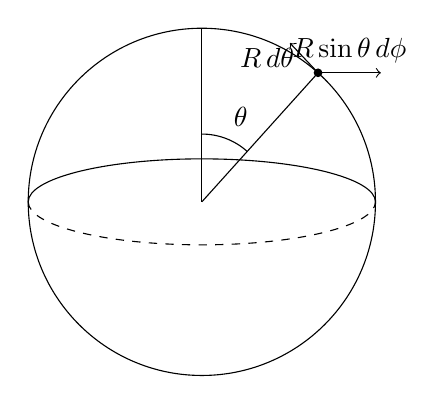
\begin{tikzpicture}[scale=1.05]
  \draw (0,0) circle (2.1);
  \draw[dashed] (-2.1,0) arc (180:360:2.1 and 0.52);
  \draw (2.1,0) arc (0:180:2.1 and 0.52);
  \coordinate (P) at (48:2.1);
  \fill (P) circle (1.5pt);
  \draw (0,0) -- (0,2.1);
  \draw (0,0) -- (P);
  \draw (0,0.82) arc (90:48:0.82);
  \node at (0.47,1.03) {\(\theta\)};
  \draw[->] (P) -- ++(-0.34,0.36)
    node[midway,left] {\(R\,d\theta\)};
  \draw[->] (P) -- ++(0.76,0)
    node[midway,above] {\(R\sin\theta\,d\phi\)};
\end{tikzpicture}
\caption{Dựng lại gọn gàng các cạnh vi phân địa phương dùng để thu được \eqref{eq:sphere-metric}.}
\end{figure}

Không có phép đổi tọa độ toàn cục nào biến \eqref{eq:sphere-metric} thành một ma trận Euclid hằng. Một quan sát viên hai chiều có thể phát hiện điều này một cách nội tại: một tam giác đủ lớn ghép từ các đường trắc địa có tổng các góc lớn hơn \(180^\circ\). Vì thế ta đã đạt tới tiêu chuẩn hữu ích. Các hệ số biến thiên tự chúng không hàm ý độ cong. Độ cong là trở ngại đối với việc tìm được các tọa độ làm cho metric hằng trên toàn bộ miền đang xét.

\section{Từ không-thời gian cong đến vũ trụ học}

Thuyết tương đối rộng cho phép chính không-thời gian mang độ cong nội tại này. Một \(g_{\mu\nu}\) phụ thuộc vị trí vẫn có thể chỉ là một tạo tác của tọa độ, như trong tọa độ cực, nhưng trong một không-thời gian thực sự cong thì không có phép biến đổi tọa độ nào loại bỏ được sự biến thiên ấy trên toàn cục.

\begin{figure}[H]
\centering
\includegraphics[width=0.70\textwidth]{lecture_08_figure_09.png}
\caption{Sự chuyển tiếp từ các ví dụ tọa độ đặc biệt sang phần tử độ dài không-thời gian tổng quát \(ds^2=g_{\mu\nu}(x)dx^\mu dx^\nu\).}
\lectureframe{00:48:40}
\end{figure}

Chúng ta sẽ không thử triển khai toàn bộ bộ máy của các phương trình Einstein. Thay vào đó, ta giới hạn sự chú ý vào các hình học thích hợp cho vũ trụ học: không gian được giả thiết là đồng nhất trên các thang đủ lớn, trong khi hình học có thể thay đổi theo thời gian. Đồng nhất có nghĩa là không có vị trí nào được ưu tiên hơn vị trí khác. Nó không có nghĩa là phẳng: mọi điểm trên một mặt cầu đều tương đương, nhưng mặt cầu vẫn cong. Nó cũng không có nghĩa là không có cấu trúc ở mọi thang.

\begin{classroomqa}
\audiencequestion{Làm sao vũ trụ có thể đồng nhất khi các thiên hà tạo thành các cụm, các tấm và các sợi?}
\lecturerresponse{Khẳng định này liên quan tới các thang được làm trơn thô. Các sao, thiên hà và cụm thiên hà là rất không đồng nhất. Khi so sánh các vùng có kích thước hàng trăm triệu năm ánh sáng, những cấu trúc đó được lấy trung bình hướng tới một phân bố đồng đều. Nguyên lý vũ trụ học là một giả thuyết làm việc có tính kinh nghiệm, không phải một tất yếu logic; những sai khác có hệ thống đủ lớn, kể cả các sai khác theo hướng trong nền vũ trụ, có thể bác bỏ nó.}
\end{classroomqa}

Giả thiết thang lớn thứ hai trong bài giảng này là tính phẳng không gian. Tại một thời gian vũ trụ cố định, các tam giác đủ lớn có vẻ Euclid: các góc của chúng cộng lại thành \(180^\circ\). Đây là một phát biểu về hình học của không gian ba chiều, chưa phải về độ cong của không-thời gian bốn chiều.

\begin{classroomqa}
\audiencequestion{Tính đồng thời có nghĩa gì đối với các điểm cách nhau bởi những khoảng cách vũ trụ học, khi ánh sáng từ chúng đến với ta ở các thời điểm khác nhau?}
\lecturerresponse{Chúng ta không thể đặt các thước đo giữa các thiên hà xa xôi hoặc quan sát chúng một cách tức thời. Ta nhận tín hiệu muộn hơn rồi tái dựng hình học của các sự kiện phát xạ trong một mô hình không-thời gian. Quy trình này là gián tiếp, nhưng nhiều phép đo hình học trong thiên văn học cũng vậy. Tính phẳng có nghĩa là các tam giác lớn được tái dựng không cho thấy phần thừa góc hay phần thiếu góc nào có thể phát hiện được trên thang đã khảo sát.}
\end{classroomqa}

\section{Tọa độ đồng chuyển động và thừa số tỉ lệ}

Hãy hình dung một lưới Descartes được vẽ lên dòng chảy thang lớn của các thiên hà. Mỗi thiên hà giữ nguyên nhãn tọa độ của mình khi lưới giãn ra. Nhãn ấy không phải là một khoảng cách tính bằng mét; nó là một địa chỉ. Một thừa số chuyển đổi phụ thuộc thời gian biến các độ tách tọa độ thành các độ tách vật lý.

\begin{figure}[H]
\centering
\begin{tikzpicture}[>=Latex,scale=0.86]
  \foreach \x in {0,0.65,1.3,1.95,2.6} {
    \draw[gray!65] (\x,0) -- (\x,2.2);
  }
  \foreach \y in {0,0.55,1.1,1.65,2.2} {
    \draw[gray!65] (0,\y) -- (2.6,\y);
  }
  \fill[blue!65!black] (0.65,0.55) circle (2pt);
  \fill[red!70!black] (1.95,1.65) circle (2pt);
  \node[below] at (1.3,-0.2) {comoving labels at \(t_1\)};
  \draw[->,very thick] (3.0,1.1) -- (4.0,1.1)
    node[midway,above] {\(a(t)\) grows};
  \foreach \x in {4.4,5.5,6.6,7.7,8.8} {
    \draw[gray!65] (\x,0) -- (\x,2.2);
  }
  \foreach \y in {0,0.55,1.1,1.65,2.2} {
    \draw[gray!65] (4.4,\y) -- (8.8,\y);
  }
  \fill[blue!65!black] (5.5,0.55) circle (2pt);
  \fill[red!70!black] (7.7,1.65) circle (2pt);
  \node[below] at (6.6,-0.2) {same labels at \(t_2\)};
\end{tikzpicture}
\caption{Các địa chỉ đồng chuyển động giữ nguyên, trong khi khoảng cách vật lý của lưới tọa độ tăng lên.}
\end{figure}

Tính đồng nhất không gian đòi hỏi cùng một thừa số chuyển đổi ở mọi nơi tại một thời điểm cho trước. Tính phẳng không gian cho phép phần không gian của metric có dạng Descartes. Phần tử độ dài thu được là
\begin{equation}
  d\tau^2
  =dt^2-a^2(t)\left(dx^2+dy^2+dz^2\right).
  \label{eq:flrw-flat}
\end{equation}
Đây là metric vũ trụ học đồng nhất phẳng theo không gian trong tọa độ đồng chuyển động. Ta có thể chọn \(x,y,z\) không thứ nguyên và cho \(a(t)\) đơn vị độ dài. Một quy ước khác có thể đưa thứ nguyên vào các tọa độ và làm cho \(a\) không thứ nguyên; chỉ tích của chúng mới quan trọng.

\begin{figure}[H]
\centering
\includegraphics[width=0.76\textwidth]{lecture_08_figure_10.png}
\caption{Metric vũ trụ học phẳng theo không gian như đã được hoàn tất trên bảng, với thừa số chung \(a^2(t)\) nhân lên cả ba phương không gian.}
\lectureframe{01:03:15}
\end{figure}

Nếu \(a\) là hằng số, ta có thể hấp thụ nó bằng cách đổi tỷ lệ \(x,y,z\), và \eqref{eq:flrw-flat} sẽ là không-thời gian Minkowski thông thường với các đơn vị khác đi. Sự phụ thuộc theo thời gian của nó mới là thành phần không tầm thường.

\begin{classroomqa}
\audiencequestion{Nếu lưới tọa độ giãn nở, tại sao thước mét, nguyên tử và các thiên hà lại không giãn nở cùng nó?}
\lecturerresponse{Metric mô tả dòng chảy vũ trụ trung bình, không phải một lực buộc mọi hệ liên kết phải đi theo nó. Lực điện từ giữ cho thước mét và nguyên tử kết dính; tự hấp dẫn giữ cho một thiên hà kết dính. Những hiệu ứng liên kết đó lấn át sự giãn nở nền cực kỳ yếu ở các thang nhỏ. Các thiên hà ở gần cũng có thể lệch khỏi dòng Hubble: Andromeda bị kéo về phía Ngân Hà. Các nghiên cứu chi tiết về sự liên kết hấp dẫn của thiên hà cho thấy chỉ riêng vật chất khả kiến là không đủ, đó là một trong những lập luận ủng hộ vật chất tối.}
\end{classroomqa}

\begin{classroomqa}
\audiencequestion{Vì sao thừa số tỉ lệ bản thân nó không phải là một lực đẩy các thiên hà ra xa nhau?}
\lecturerresponse{Theo quy ước hiện tại, nó có thứ nguyên độ dài, chứ không phải lực. Hãy nghĩ đến một viên đạn đại bác được bắn lên cao. Một khi đã được phóng đi, chuyển động hướng ra ngoài của nó là chuyển động quán tính; hấp dẫn làm thay đổi chuyển động đó bằng cách giảm tốc của nó hoặc kéo nó trở lại. Tương tự, sự giãn nở là một trạng thái chuyển động. Câu hỏi động lực học là hấp dẫn và các nguồn khác làm thay đổi \(\dot a\) và \(\ddot a\) như thế nào, chứ không phải cần lực gì để duy trì chuyển động của \(a\).}
\end{classroomqa}

Kỳ vọng trước đây là hấp dẫn hút phải làm chậm sự giãn nở. Đến thời điểm của bài giảng này, bằng chứng thiên văn đã cho thấy thay vào đó sự giãn nở gần đây đang tăng tốc, điều đó có nghĩa là động lực học đầy đủ chứa nhiều hơn vật chất hút thông thường. Ta hoãn vấn đề ấy cho đến khi thiết lập hình học đã vững chắc.

\section{Định luật Hubble}

Lấy hai thiên hà đồng chuyển động có độ tách tọa độ cố định là \(\Delta x\). Tại cùng một thời gian vũ trụ, khoảng cách vật lý của chúng là
\begin{equation}
  D(t)=a(t)\,\Delta x.
  \label{eq:physical-distance}
\end{equation}
Lấy đạo hàm trong khi giữ cố định các nhãn đồng chuyển động:
\begin{align}
  V(t)
    &=\dot D(t)
      =\dot a(t)\,\Delta x \nonumber\\
    &=\frac{\dot a(t)}{a(t)}D(t).
  \label{eq:hubble-derivation}
\end{align}
Định nghĩa
\begin{equation}
  H(t)=\frac{\dot a(t)}{a(t)}.
  \label{eq:hubble-parameter}
\end{equation}
Khi đó
\begin{equation}
  V(t)=H(t)D(t).
  \label{eq:hubble-law}
\end{equation}
Tại một thời gian vũ trụ cho trước, cùng một \(H(t)\) áp dụng ở mọi nơi; nếu không, không gian sẽ không đồng nhất. Vận tốc lùi tỉ lệ với khoảng cách vì mọi khoảng trên lưới đồng chuyển động đều bị kéo giãn với cùng một tốc độ tương đối.

\begin{figure}[H]
\centering
\includegraphics[width=0.73\textwidth]{lecture_08_figure_11.png}
\caption{Khoảng cách vật lý \(D=a\Delta x\) và đạo hàm theo thời gian của nó, trên đường dẫn tới \(V=(\dot a/a)D\).}
\lectureframe{01:16:45}
\end{figure}

\begin{classroomqa}
\audiencequestion{Đối với một thiên hà ở xa, nên lấy giá trị của tham số Hubble ở hiện tại hay tại lúc ánh sáng quan sát được đã được phát ra?}
\lecturerresponse{Tại thời kỳ đang được mô tả. Ánh sáng từ một thiên hà ở xa cho biết một giá trị sớm hơn của sự giãn nở. Một phân tích nghiêm túc phải tính đến sự phụ thuộc theo thời gian của \(H\); việc thay giá trị hôm nay vào mọi nơi chỉ là một xấp xỉ cục bộ.}
\end{classroomqa}

\begin{classroomqa}
\audiencequestion{Các đơn vị nằm ở đâu trong \(D=a\Delta x\)?}
\lecturerresponse{Một lựa chọn thuận tiện là coi nhãn đồng chuyển động \(\Delta x\) là không thứ nguyên và để \(a\) mang thứ nguyên độ dài. Cũng có thể phân bổ đơn vị theo cách ngược lại. Dù theo cách nào, \(H=\dot a/a\) có thứ nguyên nghịch đảo thời gian.}
\end{classroomqa}

\section{Ánh sáng trong hệ tọa độ giãn nở}

Ánh sáng đi theo một quỹ đạo null. Dọc theo một quỹ đạo như vậy, khoảng thời gian riêng bằng không:
\begin{equation}
  d\tau^2=0.
\end{equation}

\begin{classroomqa}
\audiencequestion{Vì sao khoảng này bằng không đối với ánh sáng?}
\lecturerresponse{Đó là hình học định nghĩa của một tia sáng trong thuyết tương đối. Mọi quan sát viên rơi tự do cục bộ đều đo được ánh sáng chuyển động với \(c=1\), nên cục bộ \(dt^2=d\ell^2\) và khoảng không-thời gian bằng không. Điều đó không có nghĩa là không có thời gian tọa độ nào trôi qua đối với quan sát viên nhận ánh sáng.}
\end{classroomqa}

Đối với một tia chỉ chuyển động theo hướng \(x\),
\begin{equation}
  0=dt^2-a^2(t)\,dx^2.
\end{equation}
Chọn tia chuyển động theo chiều \(x\) tăng,
\begin{equation}
  dt=a(t)\,dx,
  \qquad
  dx=\frac{dt}{a(t)},
  \qquad
  \frac{dx}{dt}=\frac{1}{a(t)}.
  \label{eq:null-ray}
\end{equation}

\begin{figure}[H]
\centering
\includegraphics[width=0.64\textwidth]{lecture_08_figure_12.png}
\caption{Điều kiện null trong metric giãn nở và phương trình tia sáng trong tọa độ đồng chuyển động suy ra \(dx=dt/a(t)\).}
\lectureframe{01:23:45}
\end{figure}

Vận tốc tọa độ \(dx/dt\) giảm khi thừa số tỉ lệ tăng. Điều này không có nghĩa là ánh sáng chậm đi một cách cục bộ. Một đơn vị khoảng cách tọa độ đồng chuyển động biểu diễn một khoảng cách vật lý ngày càng lớn hơn, nên giá trị số của vận tốc tọa độ thay đổi trong khi mọi phép đo cục bộ vẫn cho \(c=1\).

\section{Vì sao sự phụ thuộc theo thời gian lại quan trọng}

Câu hỏi hình học trung tâm giờ đây không thể né tránh: \(a(t)\) biến thiên như thế nào? Phép tương tự là một vật phóng mà ta biết vị trí của nó tại một thời điểm. Quỹ đạo tương lai của nó đòi hỏi một phương trình chuyển động. Trong vũ trụ học, động lực học hấp dẫn sẽ cung cấp phương trình cho \(a(t)\).

\begin{classroomqa}
\audiencequestion{Tại sao lại ưu tiên câu hỏi liệu \(a(t)\) có thay đổi hay không hơn là câu hỏi cũng chính đáng không kém rằng, chẳng hạn, điện tích electron có thay đổi theo thời gian hay không?}
\lecturerresponse{Không có thứ bậc logic nào. Một sự thay đổi đo được của điện tích electron sẽ cực kỳ quan trọng. Ta tập trung vào \(a(t)\) vì quan sát đã cho biết rằng các độ tách vũ trụ thay đổi, còn điện tích electron thì có vẻ không đổi. Về mặt hình học, một \(a\) không đổi có thể bị loại bỏ bằng một phép đổi đơn vị không gian và sẽ để lại không-thời gian phẳng; một \(a\) phụ thuộc thời gian thì không thể bị loại bỏ theo cách đó.}
\end{classroomqa}

Trước khi đo sự lùi xa ở khoảng cách lớn, cần khuôn khổ hình học này để nói rõ đang đo cái gì. Ở mức thô sơ nhất, một nguồn có độ sáng đã biết sẽ trông mờ hơn khi ở xa vì ánh sáng của nó trải ra trên một diện tích lớn hơn, còn sự dịch chuyển của các vạch phổ nguyên tử đã biết cho một độ dịch đỏ và do đó một chỉ dấu của sự lùi xa. Hubble đã kết hợp các ước lượng khoảng cách với các độ dịch đỏ để phát hiện ra tỉ lệ thuận \eqref{eq:hubble-law}, mặc dù giá trị số ban đầu của hệ số đó sai đáng kể. Các thang khoảng cách hiện đại và các phép tính lan truyền ánh sáng tương đối tính tinh vi hơn nhiều, nhưng cặp khái niệm vẫn là khoảng cách cộng với độ dịch đỏ.

\section{Thời gian Hubble và ước lượng tuổi}

Có một ước lượng đơn giản ẩn trong định luật Hubble. Hãy giữ cố định vận tốc lùi hiện tại của một thiên hà và ngoại suy chuyển động ngược về quá khứ với vận tốc đều. Thời gian cần để khép lại khoảng cách hiện tại của nó sẽ là
\begin{equation}
  t=\frac{D}{V}.
\end{equation}
Dùng \(V=HD\),
\begin{equation}
  t=\frac{D}{HD}=\frac{1}{H}.
  \label{eq:hubble-time}
\end{equation}
Khoảng cách triệt tiêu, nên mọi cặp thiên hà đồng chuyển động đều cho cùng một thời gian xấp xỉ. Susskind phát hiện và sửa một lỗi diễn đạt dễ mắc ở đây. Giả thiết không phải là \(H\) vẫn không đổi. Mà là vận tốc lùi cụ thể ấy được ngoại suy ngược về quá khứ như thể nó không đổi.

\begin{figure}[H]
\centering
\includegraphics[width=0.66\textwidth]{lecture_08_figure_13.png}
\caption{Ước lượng thời gian Hubble \(H^{-1}=D/(HD)=D/V\), trong đó khoảng cách triệt tiêu trong phép ngoại suy ngược.}
\lectureframe{01:33:45}
\end{figure}

Vì thế, nghịch đảo của tham số Hubble là một thang thời gian, chứ không tự động là tuổi chính xác của vũ trụ. Trong một mô hình thuần túy chậm dần, bị vật chất chi phối, hãy đảo ngược vận tốc hiện tại và để hấp dẫn kéo các thiên hà lại với nhau. Chúng gặp nhau sớm hơn so với trường hợp vận tốc đều, nên \(H^{-1}\) hiện nay đánh giá quá cao tuổi của vũ trụ. Bài giảng nêu một tuổi hiệu chỉnh vào khoảng \(13.5\) tỷ năm, gần với thời gian Hubble nhưng không đồng nhất với nó.

\begin{classroomqa}
\audiencequestion{Nếu không có sự giãn nở Hubble bên trong thiên hà của chúng ta, thì việc cho mọi thiên hà chạy ngược lại cho đến khi chúng sụp lại có nghĩa gì?}
\lecturerresponse{Mô tả đồng nhất rốt cuộc không còn đủ độ phân giải để phản ánh lịch sử thực của các cấu trúc liên kết. Khi tiến về phía trước theo thời gian, những dao động nhỏ lớn lên dưới tác dụng hấp dẫn thành các thiên hà và cụm thiên hà. Một bộ phim đảo ngược theo nghĩa đen sẽ đòi hỏi mọi chuyển động vi mô đều đảo chiều và entropy giảm; chỉ đơn giản đảo ngược dòng Hubble trung bình không thể hoàn tác sự hình thành cấu trúc. Phép ngoại suy ngược là một ước lượng vũ trụ học thô, không phải một bộ phim trong đó mọi ngôi sao lần theo lại đường đi của nó.}
\end{classroomqa}

\begin{classroomqa}
\audiencequestion{Liệu một thí nghiệm có thể phân biệt khoảng cách liên thiên hà đang giãn nở với một cây thước đang co lại không?}
\lecturerresponse{Chỉ các tỉ số không thứ nguyên là quan sát được. Điều được đo là khoảng cách giữa các thiên hà chia cho một chuẩn độ dài nguyên tử hoặc trong phòng thí nghiệm đang tăng lên. Theo quy ước, ta giữ cố định các tham số của vật lý nguyên tử và phân tử và nói rằng vũ trụ giãn nở. Người ta cũng có thể chọn độ tách liên thiên hà làm chuẩn và mô tả các nguyên tử, proton và thước mét là đang co lại. Vật lý của tỉ số ấy sẽ không đổi.}
\end{classroomqa}

Quy ước đó là tự nhiên vì các thanh đo được làm từ nguyên tử và kích thước của chúng được chi phối bởi các tham số dường như không đổi. Một mét rốt cuộc là một số rất lớn các độ dài vi mô. Giữ cố định các chuẩn vi mô ấy cho ta phát biểu quen thuộc rằng \(a(t)\) tăng.

\begin{classroomqa}
\audiencequestion{Có phải \eqref{eq:flrw-flat} là metric duy nhất tương thích với tính đồng nhất và tính phẳng của không gian không?}
\lecturerresponse{Chỉ đúng tới các phép biến đổi tọa độ. Phát biểu chính xác là, dưới những giả thiết đó và với một lựa chọn thích hợp về thời gian vũ trụ cùng các tọa độ không gian đồng chuyển động, metric có thể được đưa về dạng này. Một hệ tọa độ khác có thể khiến cùng một không-thời gian trông khá khác.}
\end{classroomqa}

\begin{classroomqa}
\audiencequestion{Khi độ tách trong phép ngoại suy ngược đạt tới 0, định luật Hubble cũng cho vận tốc bằng 0. Điều đó có ngăn các thiên hà gặp nhau không?}
\lecturerresponse{Không. \(H\) được suy ra hôm nay không được giữ cố định suốt ngược về quá khứ. Trong các nghiệm giãn nở thông thường, \(H(t)\) ở các thời điểm sớm hơn lớn hơn nhiều. Ước lượng \(H_0^{-1}\) được thực hiện bằng cách kéo dài đều vận tốc hôm nay chỉ để lấy một thang đo; các \(a(t)\), \(H(t)\) và các vận tốc thực sự phải được tìm từ động lực học.}
\end{classroomqa}

\section{Định lý vỏ cầu của Newton và động lực học vũ trụ học}

Để tìm ra động lực học, hãy trải đều các thiên hà thành một môi trường đồng nhất. Chọn một thiên hà làm gốc tọa độ và một thiên hà khác có nhãn đồng chuyển động \(x\). Lựa chọn này không có ưu thế vật lý nào; tính đồng nhất đòi hỏi phương trình cuối cùng phải như nhau quanh mọi thiên hà. Bán kính vật lý của thiên hà thứ hai là
\begin{equation}
  R(t)=a(t)x.
  \label{eq:radius-ax}
\end{equation}

Thoạt đầu, việc tìm gia tốc hấp dẫn của nó dường như đòi hỏi phải cộng lực hút của mọi thiên hà trong một vũ trụ khổng lồ. Định lý vỏ cầu của Newton rút gọn bài toán này:

\begin{proposition}[Newton's shell theorem]
Đối với một lực nghịch đảo bình phương và một phân bố khối lượng đối xứng cầu, vật chất ở ngoài mặt cầu đi qua điểm thử đóng góp lực tổng cộng bằng không. Vật chất bên trong mặt cầu tác dụng lên điểm thử như thể toàn bộ khối lượng bị bao chứa tập trung tại tâm.
\end{proposition}

\begin{figure}[H]
\centering
\includegraphics[width=0.70\textwidth]{lecture_08_figure_14.png}
\caption{Phân bố thiên hà đồng nhất, một thiên hà thử tại nhãn đồng chuyển động \(x\), và mặt cầu mà chỉ khối lượng chứa bên trong nó mới chi phối chuyển động xuyên tâm của thiên hà ấy.}
\lectureframe{01:50:05}
\end{figure}

\begin{figure}[H]
\centering
\begin{tikzpicture}[scale=0.94,>=Latex]
  \draw[gray!65] (0,0) circle (2.35);
  \foreach \p in {
    (-1.5,0.8),(-1.2,-0.8),(-0.8,1.5),(-0.6,0.35),(-0.3,-1.45),
    (0.15,1.05),(0.35,-0.55),(0.7,1.65),(0.9,0.45),(1.25,-0.9),
    (1.65,0.95),(-1.75,-0.2),(1.8,-0.15)} {
    \fill[black!55] \p circle (1.15pt);
  }
  \fill[blue!65!black] (0,0) circle (2pt)
    node[below left] {chosen origin};
  \fill[red!70!black] (2.35,0) circle (2.2pt)
    node[right] {test galaxy};
  \draw[->,thick] (0,0) -- (2.32,0)
    node[midway,above] {\(R=a(t)x\)};
  \draw[<->] (-2.35,-2.55) -- (2.35,-2.55)
    node[midway,below=4pt] {only the enclosed mass contributes};
\end{tikzpicture}
\caption{Dựng lại gọn gàng bố trí của định lý vỏ cầu. Gốc tọa độ là một lựa chọn thuận tiện, không phải tâm của vũ trụ.}
\end{figure}

Vì thế bài toán nhiều vật thể trong vũ trụ học đã trở thành một bài toán một vật thể quen thuộc: một vật phóng chuyển động theo phương xuyên tâm dưới lực hút của khối lượng chứa bên trong mặt cầu hiện tại của nó. Phương trình Newton sẽ xác định \(R=a x\), và do đó \(a(t)\), gia tốc ra sao. Bài giảng cố ý dừng lại trước khi thực hiện phép tính đó. Buổi sau sẽ suy ra mô hình vũ trụ học đơn giản nhất bị vật chất chi phối, thay vì lén đưa đáp án của nó vào trong phần thiết lập hình học.

\section{Các câu hỏi cuối: ánh sáng, Vụ Nổ Lớn và độ cong}

Bài giảng chính thức đã kết thúc, nhưng các câu hỏi cuối cùng phơi bày vài hình dung dễ gây hiểu lầm và là một phần của vật lý chứ không phải một phụ lục.

\begin{classroomqa}
\audiencequestion{Nếu ánh sáng từ các vật thể rất xa được phát ra khi
vũ trụ còn nhỏ hơn nhiều, thì vì sao nay nó lại có vẻ như đến từ xa đến vậy?
Và nếu vũ trụ sơ khai là nhỏ gọn, thì vì sao không phải toàn bộ nó đều quan sát được?}
\lecturerresponse{Ta phải giải phương trình tia null trong các tọa độ giãn nở. Khi \(a(t)\) rất nhỏ, \(dx/dt=1/a(t)\) rất lớn:
ánh sáng đi qua một khoảng đồng chuyển động lớn trong khi cục bộ vẫn chuyển động với
\(c=1\). Khi \(a(t)\) tăng, vận tốc tọa độ đồng chuyển động của nó giảm. Điểm
phát ra chính xác và kích thước của vùng quan sát được phụ thuộc vào toàn bộ
lịch sử của \(a(t)\), nên câu trả lời bằng số được hoãn lại cho đến khi giải
xong một mô hình vũ trụ học cụ thể.}
\end{classroomqa}

\begin{figure}[H]
\centering
\includegraphics[width=0.72\textwidth]{lecture_08_figure_15.png}
\caption{Một tia sáng trong mặt phẳng \((x,t)\): gần như nằm ngang trong tọa độ
đồng chuyển động khi \(a(t)\) nhỏ, rồi dốc dần hơn khi thừa số tỉ lệ tăng.}
\lectureframe{01:56:20}
\end{figure}

Lấy tích phân \eqref{eq:null-ray} sẽ viết tường minh phép tính đã được hoãn lại:
\begin{equation}
  \Delta x
  =\int_{t_{\mathrm e}}^{t_0}\frac{dt}{a(t)}.
  \label{eq:comoving-light-distance}
\end{equation}
Việc tích phân có đạt tới các khoảng cách đồng chuyển động lớn tùy ý khi
\(t_{\mathrm e}\) tiến về thời điểm ban đầu hay không phụ thuộc vào dạng ở thời sớm
của \(a(t)\).\editorialnote{Phương trình \eqref{eq:comoving-light-distance} là
dạng đã tích phân của phương trình trên bảng \(dx=dt/a(t)\). Nó viết tường minh
phép tính mà bài giảng giao cho buổi sau mà không chọn một thừa số tỉ lệ cụ
thể.}

\begin{figure}[H]
\centering
\begin{tikzpicture}[scale=0.92,>=Latex]
  \draw[->] (0,0) -- (6.4,0) node[right] {\(x\)};
  \draw[->] (0,0) -- (0,4.6) node[above] {\(t\)};
  \draw[thick,blue!65!black]
    plot[smooth] coordinates {(0,0.18) (1.65,0.42) (2.65,1.05)
      (3.35,2.05) (3.85,3.25) (4.05,4.25)};
  \fill[red!70!black] (4.05,4.25) circle (2pt)
    node[right] {reception today};
  \draw[dashed] (4.05,0) -- (4.05,4.25);
  \node[align=left] at (1.65,3.25)
    {\(\displaystyle \frac{dx}{dt}=\frac1{a(t)}\)\\
     large when \(a\) is small};
\end{tikzpicture}
\caption{Bản gọn của cách dựng tia sáng trong tọa độ đồng chuyển động. Độ dốc thay đổi
là một hiệu ứng tọa độ, không phải sự thay đổi của tốc độ ánh sáng cục bộ.}
\end{figure}

\begin{classroomqa}
\audiencequestion{Vụ Nổ Lớn có bắn vật chất ra từ một điểm, để đến nay nó phải nằm trên
một vỏ hay một vòng đang giãn nở không?}
\lecturerresponse{Không. Mô hình bắt đầu với một không gian đồng nhất, cực kỳ đậm
đặc. Mọi khoảng cách ở thang lớn đều tăng; vật chất không bị phóng qua
không gian trống tồn tại sẵn từ một tâm ưu tiên. Một quả bóng bay được phủ đều các
chấm là một phép tương tự hai chiều hữu ích: khi nó nở ra, mọi khoảng cách
giữa các chấm đều tăng trong khi bề mặt vẫn được phủ đều. Không gian thậm
chí có thể là vô hạn ở mọi thời điểm dương; sự giãn nở không hàm ý rằng nó
đã bắt đầu như một quả cầu hữu hạn nằm bên trong một thứ gì khác.}
\end{classroomqa}

\begin{classroomqa}
\audiencequestion{Bản thân hấp dẫn trong quá trình giãn nở là yếu hơn hay mạnh hơn?}
\lecturerresponse{Trong phần thảo luận này, hằng số Newton \(G\) được giữ cố định. Tuy vậy,
lực vẫn thay đổi vì các khoảng cách và các mật độ bên trong thay đổi. Ở các
thời điểm sớm hơn, cùng thiên hà đồng chuyển động ấy ở gần hơn về mặt vật lý
và vật chất đồng nhất đặc hơn, nên độ giảm tốc do hấp dẫn lớn hơn. Đây chính
là điều mà phép tính định lý vỏ cầu nhằm định lượng.}
\end{classroomqa}

Cuối cùng, không được nhầm độ cong không gian với sự giãn nở. Một vùng nhỏ
trên Trái Đất có vẻ phẳng vì kích thước của nó quá nhỏ so với bán kính Trái
Đất. Bằng cách đo các tam giác đủ lớn, người ta hoặc có thể phát hiện độ dư
góc, hoặc đặt một cận dưới cho bán kính cong. Thiên văn học làm thí nghiệm
tương tự với những tam giác khổng lồ. Trong ngôn ngữ quan sát được dùng trong
bài giảng 2006, không phát hiện thấy độ cong nào trên miền nhìn thấy,
nên bất kỳ bán kính cong nào cũng phải lớn hơn đáng kể miền đó. Điều này
không chứng minh một vũ trụ phẳng chính xác; nó chỉ giới hạn mức độ cong của
phần có thể tiếp cận.

Đối với một mặt cầu, độ cong nội tại tỉ lệ như \(R^{-2}\). Vì vậy, một mặt cầu lớn dần
trở nên phẳng hơn về mặt cục bộ. Tương tự, nếu một vũ trụ đồng nhất có độ cong
không gian khác không, sự giãn nở làm tăng bán kính cong của nó và làm giảm độ
cong nhìn thấy được trong bất kỳ miền cục bộ có kích thước cố định nào.
\editorialnote{Tỉ lệ \(R^{-2}\) là dạng định lượng chuẩn của phát biểu trong
bài giảng rằng giá trị số của độ cong giảm khi một mặt cầu lớn lên.}

\begin{classroomqa}
\audiencequestion{Nếu không gian cong, có nhất thiết một phần của vũ trụ phải co lại
trong khi phần khác giãn ra không?}
\lecturerresponse{Không. Độ cong không gian dương, bằng không hoặc âm mô tả
hình học của từng lát cắt theo thời gian vũ trụ. Sự giãn nở hay co lại được chi
phối bởi sự tiến triển của \(a(t)\). Một vũ trụ cong có thể giãn nở; một
vũ trụ phẳng có thể co lại. Sự giãn nở về sau có thể đảo chiều, cũng như một
vật được phóng lên có thể rơi trở lại, nhưng không có sự co đồng thời nào bị
ẩn trong độ cong. Vấn đề động lực học là chuyển động đi ra ngoài ấy thoát khỏi
lực hút của khối lượng bị bao, rơi trở lại, hay nằm trên ranh giới tới hạn.}
\end{classroomqa}

So sánh với vận tốc thoát đó là ý tưởng cuối cùng được trình bày trên bảng
của bài giảng. Hình học đã cung cấp metric, định luật Hubble và phương trình tia
sáng. Định lý của Newton đã quy động lực học về khối lượng bên trong một mặt
cầu. Bài giảng tiếp theo bắt đầu đúng ở chỗ bài này nên kết thúc: với phương
trình quyết định \(a(t)\), và với câu hỏi liệu sự giãn nở sẽ thoát đi, co
sụp trở lại, hay nằm đúng trên lằn ranh mong manh.
